%%%%%%%%%%%%%%%%%%%%%%%%%%%%%%%%%%%%%%%%%%%%%%%%%%%%%%%%%%
%
% Doctoral Thesis Template @ The University of Manchester
% LaTeX Chapter Template
% Version 1 (23/07/2020)
% Joe Crone
%
% This template is based on:
% The University of Manchester, Presentation of Thesis Policy
% Research Office Graduate Education Team
% June 2017
% http://www.regulations.manchester.ac.uk/pgr-presentation-theses/
%
%%%%%%%%%%%%%%%%%%%%%%%%%%%%%%%%%%%%%%%%%%%%%%%%%%%%%%%%%%
\documentclass[../main.tex]{subfiles}
\begin{document}

% Title
%--------------------------------------------------------
\chapter{CBETA Multi-Pass Commissioning}
\label{CBETA_Multi-Pass_Commissioning} % to reference use \ref{ChapterTemplate}

\section{CBETA ERL}

\section{De-Gaussing of Spreader Magnets}

\textcolor{blue}{**NEEDS PLENTY OF WORK, GETTING POINTS DOWN** \\ **NOTEBOOK 8 HAS ALL OF THE DETAILS + NOTES**}

Hysteresis effects within spreader magnets in the splitter/recombiner lines degraded the reproducibility of CBETA configurations between consecutive operational periods. Once the accelerator orbit was tuned, a series of magnet strength set points corresponding to the orbit could be saved however hysteresis invalidates the previously discovered set points.

The hysteresis effects occur because of the use of ferromagnetic materials in the yokes of magnets to enhance the magnetic field of a coil. Ferromagnetic materials used in this typically have a strong dependence on their history \cite{decker1991physical} -- previous magnetizations affect the current state of the magnet via the yoke material. An example of an anhysteretic $B$--$I$ curve of a ferromagnetic yoke material, as used in an electromagnet, is shown in Figure~\ref{fig:example_BI_curve}.

\begin{figure}[!h]
\centering
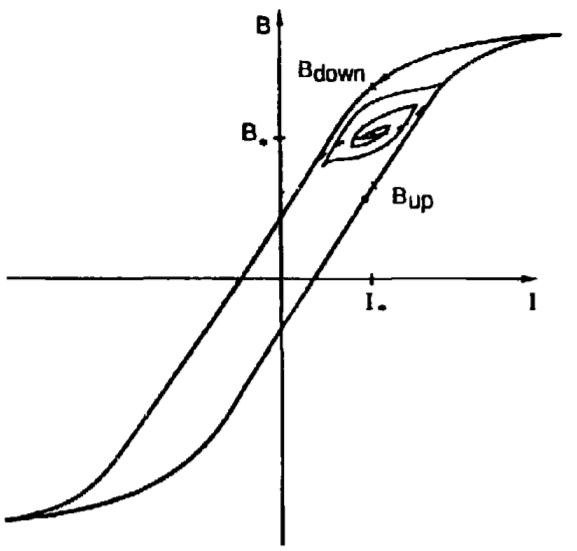
\includegraphics[width=0.7\textwidth]{Figures/CBETA_Multi-Pass_Commissioning/example_BI_curve.png}
\caption{Example $B$--$I$ anhysteric curve of a ferromagnetic yoke material \cite{decker1991physical} \textcolor{blue}{don't know what else to say}}
\label{fig:example_BI_curve}
\end{figure}

\textcolor{blue}{**WRITE HOW DEGAUSSING WORKS VIA THE STEVE PEGGS NOTE**}

The basic procedure is to repetitively alternate the current passed through the coils of the magnet around the tuning set point thereby increasing and decreasing the induced magnetic field. This shifts the position in the $B$--$H$ (or $B$--$I$) hysteresis curve upon which the magnet lies and instead leads to the magnet following its original $B$--$H$ curve. \textcolor{blue}{**Explanation needs a lot of work**} The original trialed procedure was based upon the procedure used for a series of quadrupoles at LCLS \cite{weidemann2010degaussing}.   

\begin{equation}
I\left(t\right) = I_{0}+\Delta I\exp\left(-t/\tau\right)\sin\left(\omega t\right),
\label{eq:decker_degauss_current}
\end{equation}
where $I_{0}$ is the magnet set point current, $\Delta I$ is the swing current by which the magnet current is varied, $\tau$ is the pause time between current variations, $t$ is the time from initiation of the procedure and $\omega$ is \textcolor{blue}{I don't know...}. 

Converted into a set of cycles with a two second pause in between each cycle, the current of any cycle number $n_{\mathrm{cycle}}$ can be wrote as
\begin{equation}
I\left(n_{\mathrm{cycle}}\right) =  I_{0}+\Delta I\left(-1\right)^{n_{\mathrm{cycle}}}\left(1-\kappa\right),
\label{eq:cycle_degauss_current_fractional}
\end{equation}
where $\kappa$ is the fractional decrease in swing current as given by
\begin{equation}
\kappa = \frac{n_{\mathrm{cycles}}}{n_{\mathrm{tot}}},
\label{eq:fractional_swing_current_decrease}    
\end{equation}
with $n_{\mathrm{tot}}$ the total number of cycles performed in the de-gaussing procedure.

In practice the de-gaussing procedure is applied to all spreader magnets and correctors simultaneously as the de-gaussing procedure enacted upon each magnet takes $\sim t_{\mathrm{pause}n_{\mathrm{tot}}}$ to run. With the large number of magnets \textcolor{blue}{how many spreader magnets?} and vast number of correctors \textcolor{blue}{how many?} it would be time prohibitive to run these consecutively. However, this has the notable drawback of enabling cross-talk between neighbouring magnets during the de-gaussing procedure which may impact efficacy.

\textcolor{blue}{**WRITE ABOUT HOW $\Delta I$ IS DEFINED AND ITS DRIVE HIGH/LOW LIMITS**}
The swing current $\Delta I$ in (Eq.~\ref{eq:cycle_degauss_current_fractional}) varies based on the set point current of the magnet $I_{0}$ and the current limitations of the magnet in question, named the drive high current $I_{\mathrm{DRVH}}$ which is the maximum tolerable current and the drive low current $I_{\mathrm{DRVL}}$ which is the minimum tolerable current (typically zero for non-bipolar magnets). Therefore, the sing current can be represented as
\begin{equation}
\Delta I =
\begin{cases}
\left|I_{0}-I_{\mathrm{DRVL}}\right|, \text{ if odd} \\
\left|I_{0}-I_{\mathrm{DRVH}}\right|, \text{ if even.}
\end{cases}
\label{eq:swing_current_variation}
\end{equation}
For example, for a bi-polar corrector coil the current tolerance is $\pm 3$~\si{\ampere}, which corresponds to the drive high and drive low currents, and these correctors typically have a set point current of $I_{0} = 0$~\si{\ampere} (as we aim to operate without magnetic correction) so the swing current in this case is $\Delta I = 3$~\si{\ampere}.     

\textcolor{blue}{**SHOW I--t PLOT OF BOTH THE FRACTIONAL AND MIN MAX PROCEDURES** \\ plot $t_{\mathrm{pause}}$ as time for varying current, do for a single magnet with defined $\Delta I$}

Steve Peggs has looked into de-gaussing of the CBETA H1 dipole magnets \cite{fabus2019hysteresis}

In order to increase reproducibility of the CBETA ERL configuration during commissioning a script was devised to combat the hysteresis effects by 'de-Gaussing' the magnets within the splitter lines. Only the splitter line magnets were initially selected as this procedure is only applicable to electromagnets; the FFA magnets are permanent magnet quadrupoles and combined function magnets. However, this was eventually extended to the window frame corrector coils on the FFA permanent magnets.

The more complicated procedure detailed here was abandoned after testing because it failed to accomplish full de-gaussing of the spreader magnets. The Max to Zero scheme outlined by Fabus and Peggs \cite{fabus2019hysteresis}, though applied to more than the H1 dipoles, was found to be more easily applicable and effective. This involved repetitively driving the power supply to produce the maximum and minimum current within its tolerable limits to produce the maximum and minimum magnetic flux density. Typically this involves a maximum to zero current variation however for bipolar magnets this involved alternating the sign of the maximum magnitude of the magnetic flux density. In this case, as opposed to the fractional variation of current (Eq.~\ref{eq:cycle_degauss_current_fractional}), the current is varied per cycle as
\begin{equation}
I\left(n_{\mathrm{cycle}}\right) =  I_{0}+\Delta I\left(-1\right)^{n_{\mathrm{cycle}}},
\label{eq:cycle_degauss_current_max_min}
\end{equation}
where the $\left(1-\kappa\right)$ term in (Eq.~\ref{eq:cycle_degauss_current_fractional}) is abandoned.

\begin{figure}[!h]
\centering
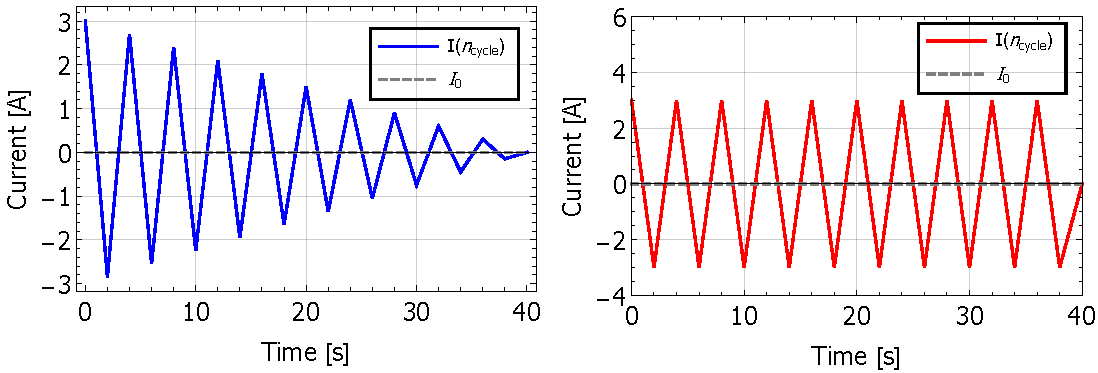
\includegraphics[width=\textwidth]{Figures/CBETA_Multi-Pass_Commissioning/degauss_current_time_corrector.pdf}
\caption{Plots of de-Gaussing procedures in current--time ($I$--$t$) space for the permanent magnet window frame correctors. The correctors are typically operated using bi-polar power supplies with a $I_{\mathrm{DRVH/DRVL}}=\pm3$~\si{\ampere} current limit and their set point is $I_{0}=0$~\si{\ampere} as for nominal operation correctors should not be necessary. Current is varied in $t_{\mathrm{pause}}=2$~\si{\second} intervals for a total of $n_{\mathrm{tot}}=20$ cycles. Left: Fractional de-Gaussing method (Eq.~\ref{eq:cycle_degauss_current_fractional}). Right: Min to Zero de-Gaussing method (Eq.~\ref{eq:cycle_degauss_current_max_min}). }
\label{fig:corrector_degauss_procedure}
\end{figure}

\begin{figure}[!h]
\centering
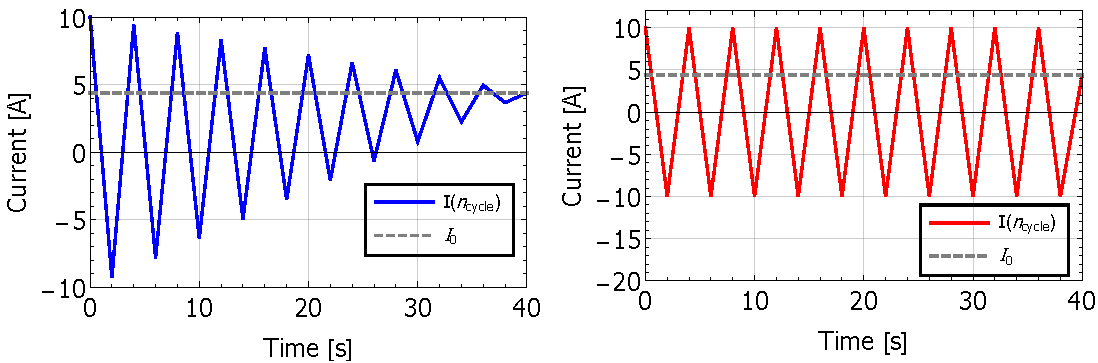
\includegraphics[width=\textwidth]{Figures/CBETA_Multi-Pass_Commissioning/degauss_current_time_MS1QUA02.pdf}
\caption{Plots of de-Gaussing procedures in current--time ($I$--$t$) space for the MS1QUA02 quadrupole located in the S1 spreader line. The MS1QUA02 operated using a bi-polar power supply with a $I_{\mathrm{DRVH/DRVL}}=\pm10$~\si{\ampere} current limit and a set point current of $I_{0}=4.39$~\si{\ampere}. Current is varied in $t_{\mathrm{pause}}=2$~\si{\second} intervals for a total of $n_{\mathrm{tot}}=20$ cycles. Left: Fractional de-Gaussing method (Eq.~\ref{eq:cycle_degauss_current_fractional}). Right: Min to Zero de-Gaussing method (Eq.~\ref{eq:cycle_degauss_current_max_min}).}
\label{fig:MS1QUA02_degauss_procedure}
\end{figure}

\begin{figure}[!h]
\centering
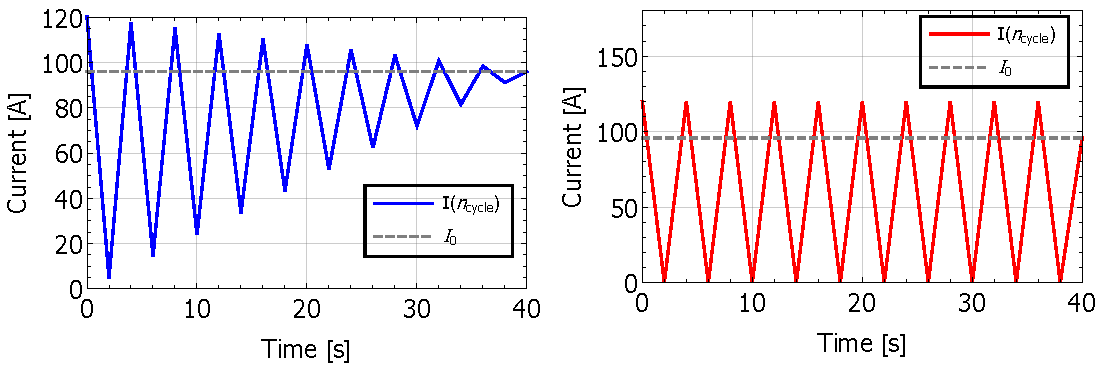
\includegraphics[width=\textwidth]{Figures/CBETA_Multi-Pass_Commissioning/degauss_current_time_MS1DIP03.pdf}
\caption{Plots of de-Gaussing procedures in current--time ($I$--$t$) space for the MS1DIP03 dipole in the S1 (42~\si{\mega\electronvolt}) spreader line. The correctors are typically operated using a power supply with a $I_{\mathrm{DRVH}}=120$~\si{\ampere} maximum current limit ($I_{\mathrm{DRVL}}=0$) and their set point is $I_{0}=95.93$~\si{\ampere}. Current is varied in $t_{\mathrm{pause}}=2$~\si{\second} intervals for a total of $n_{\mathrm{tot}}=20$ cycles. Left: Fractional de-Gaussing method (Eq.~\ref{eq:cycle_degauss_current_fractional}). Right: Min to Zero de-Gaussing method (Eq.~\ref{eq:cycle_degauss_current_max_min}).}
\label{fig:MS1DIP03_degauss_procedure}
\end{figure}

\section{Multi-pass FFA Chromaticity Measurement}

\textcolor{blue}{**AGAIN, JUST GETTING POINTS DOWN HERE** \\ **NOTEBOOK 9 HAS CHROMATICITY NOTES, POSITIONS MARKED BY POST-IT**}

A measurement script has been developed and tested, with experiment during CBETA commissioning, to measure the chromaticity per cell (in both planes) of sections of the CBETA FFA recirculation line, for all 4 turns. Chromaticity per cell $Q'_{x/y}$ can be experimentally measured through measurement of the tune per cell $Q_{x/y}$ as a function of the relative change in momentum of an electron beam $\delta p/p$, as shown in (Eq.~\ref{eq:chromaticity_measurement_central})
\begin{equation}
\Delta Q = Q'\frac{\delta p}{p}.
\label{eq:chromaticity_measurement_central}
\end{equation}
In practice this was accomplished by recursively applying a modified version of an existing script used to measure tune in sections of the FFA whilst incrementing the electron beam energy, thereby changing the electron momentum spread $\Delta p/p$. Firstly, a history of previous ERL chromaticity measurements is presented, then details of this measurement are outlined in Section~\ref{sec:chromaticity_measurement_methodology}, then experimental results are shown in Section~\ref{sec:CBETA_chromaticity_measurement_results}. Finally, the results of this approach are discussed in Section~\ref{sec:chromaticity_discussion}. 

\subsection{ERL Chromaticity Measurements}
\label{sec:ERL_chromaticity_measurements}

Chromaticity measurements within non-scaling FFA transport and for multi-pass ERLs have never been successfully accomplished \textcolor{blue}{**CHECK**}

\textcolor{blue}{**LITERATURE REVIEW SECTION** \\ What was the original source I used for this? }

\subsection{Chromaticity Measurement Methodology}
\label{sec:chromaticity_measurement_methodology}

The energy of a particle after traversing an RF cavity is given by
\begin{equation}
E_{e} = qV_{\mathrm{RF}}\sin\phi_{\mathrm{RF}},
\label{eq:particle_acceleration_energy}
\end{equation}
where $q$ is the charge of the particle (we consider only electrons, $q=e$), $V_{\mathrm{RF}}$ is the maximum RF cavity voltage (generator voltage) and $\phi_{\mathrm{RF}}$ is the RF accelerating phase the electron bunch witnesses. From inspection of (Eq.~\ref{eq:particle_acceleration_energy}), it is possible to vary the energy of the electron bunch in two main ways: by varying the maximum RF cavity voltage or through variation of the accelerating phase. For the chromaticity measurement on CBETA the energy of the electron bunch was manipulated through adjustment of cavity 1 voltage (the cavity traversed last by an accelerated beam). The electron momentum spread is related to the change in RF cavity generator voltage by
\begin{equation}
\frac{\Delta p}{p}\approx \frac{\Delta E_{e}}{E_{e}} = \frac{\Delta V_{\mathrm{RF}}}{V_{\mathrm{RF}}}.    
\end{equation}

To measure the \textcolor{blue}{fractional?} tune per cell of a section of CBETA a vertical or horizontal kick is generated to cause a betatron oscillation which propagates through the FFA common transport return line \cite{gulliford2021measurement}. The vertical kick is provided by the last vertical corrector in the corresponding splitter line of that turn; for example, the 3rd turn vertical kick is provided by the MS3CRV04 vertical corrector. Horizontal kicks are implemented by the last independent dipole magnet (non-septa) in which only a single bunch is traverses the magnet as otherwise betatron oscillations would be generated cumulatively in each effected turn. Quality of orbit kicks in CBETA is also affected by cross-talk between magnets therefore dipole selection is also dependent upon this condition \textcolor{blue}{**IMPROVE THIS SENTENCE**}. For example, the MS2DIP08 dipole is used to induce a horizontal kick in the 78~\si{\mega\electronvolt} 2nd turn. Within an ERL the bunch will traverse the splitter line in each turn twice (with the exception of the 4th turn) passing through in both accelerating and decelerating configuration therefore two kicks are applied to a bunch \textcolor{blue}{How is this problem -- if it is a problem -- solved?}.     

The closed orbit throughout the whole accelerator is modulated via the induced betatron oscillation which is measured by the beam position monitors (BPMs) in the FFA which can detect variation in bunch position in either transverse plane. As per the procedure used in the CBETA fractional arc test \cite{gulliford2019beam} -- a preliminary investigation of FFA transport arcs -- the BPM data is analysed by fitting of a sinusoidal function \textcolor{blue}{**EXPAND**} to produce the betatron phase advance per cell given by
\begin{equation}
\Psi_{x/y}\left(s\right) = \int_{0}^{s}\frac{1}{\beta_{x/y}\left(s\right)}ds,
\label{eq:betatron_phase_advance_per_cell}
\end{equation}
where $s$ is the distance traversed for a single cell in the direction of propagation and $\beta_{x/y}\left(s\right)$ is the $\beta$-function, the amplitude of this oscillation. The betatron phase advance per cell can then be converted into tune per cell via 
\begin{equation}
Q_{x/y} = \frac{1}{2\pi}\int_{0}^{s} \frac{1}{\beta_{x/y}\left(s\right)}ds.
\label{eq:tune_definition}
\end{equation}

\subsection{CBETA Chromaticity Measurement Results}
\label{sec:CBETA_chromaticity_measurement_results}

The chromaticity and tune per cell of the FFA can be predicted via \textsc{Opera} fieldmap tracking simulations. \textcolor{blue}{**ASK KIRSTEN WHERE THIS IS FROM**} Data for the fieldmap tracking simulations of the FA/FB arcs and the ZX straight have been made available by the CBETA collaboration. \textcolor{blue}{**WHAT ARE THE I and H DATA SETS--ASK KIRSTEN**} The tune data has bee converted into chromaticity data via a re-arrangement of (Eq.~\ref{eq:chromaticity_measurement_central}), with appropriate substitution of the total electron beam energy
\begin{equation}
Q'_{x/y} = \frac{\Delta Q E_{e}}{\Delta E_{e}}.
\label{eq:fieldmap_chromaticity}
\end{equation}
The plots of the chromaticity and tune per cell in each plane from fieldmap tracking simulations for the CBETA FFA sections (FA/FB arc and ZX straight) are shown in Fig.~\ref{fig:fieldmap_chromaticity_tune} for a 40--160~\si{\mega\electronvolt} electron bunch energy range.
\begin{figure}[!h]
\centering
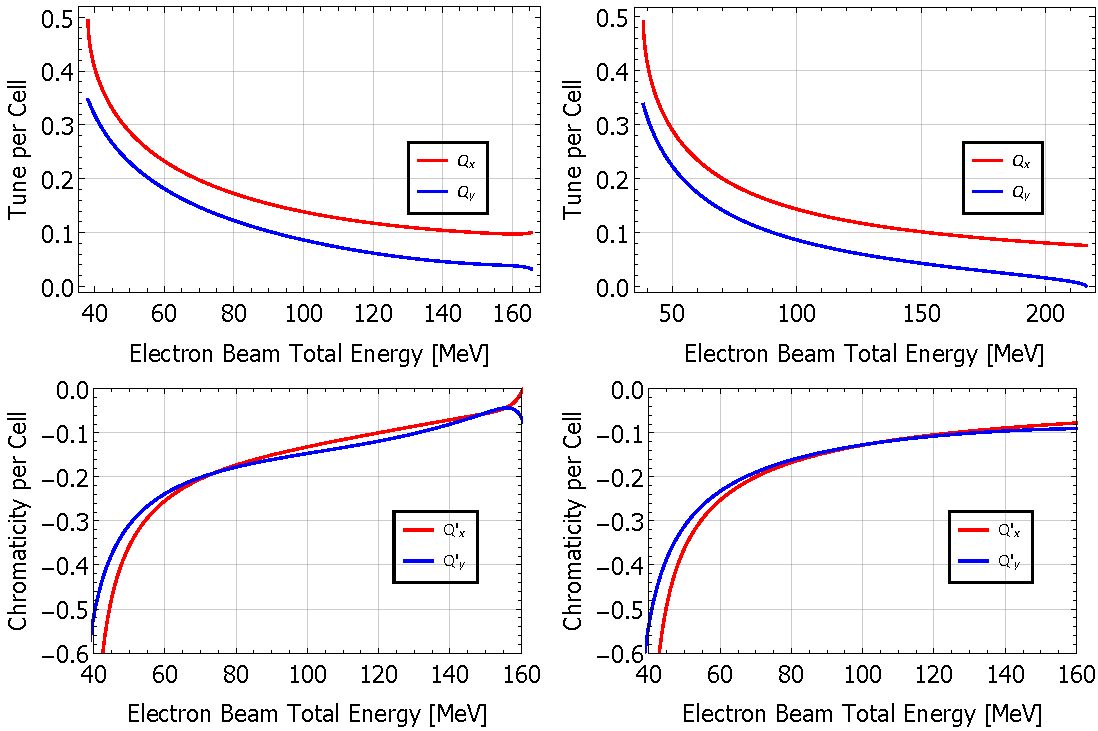
\includegraphics[width=\textwidth]{Figures/CBETA_Multi-Pass_Commissioning/fieldmap_grid.pdf}
\caption{CBETA fieldmap tracking simulations as a function of electron beam total energy. Top Left: FA/FB arc tune per cell in each transverse plane. Top Right: ZX straight tune per cell in each plane. Bottom Left: Chromaticity per cell of the FA/FB arc in each transverse plane. Bottom Right: ZX straight chromaticity per cell in each plane. }
\label{fig:fieldmap_chromaticity_tune}
\end{figure}

\subsection{Discussion}
\label{sec:chromaticity_discussion}

Unfortunately, this script was only tested on the last day of operation; due to energy drift in the linac only measurements
up to the second turn produced usable data when this was compared to the expected tune produced from fieldmap tracking.


\end{document}